\section{变阻器}\label{sec:8-10}

在生产和实验中,常用改变电阻的方法来控制电路中的电流强度。
从前面一节的研究知道,如果改变导体的长度,它的电阻也跟着改变。
变阻器就是靠改变电路中电阻线的长度来改变电阻,从而改变电流强度的。

\begin{figure}[htbp]
    \centering
    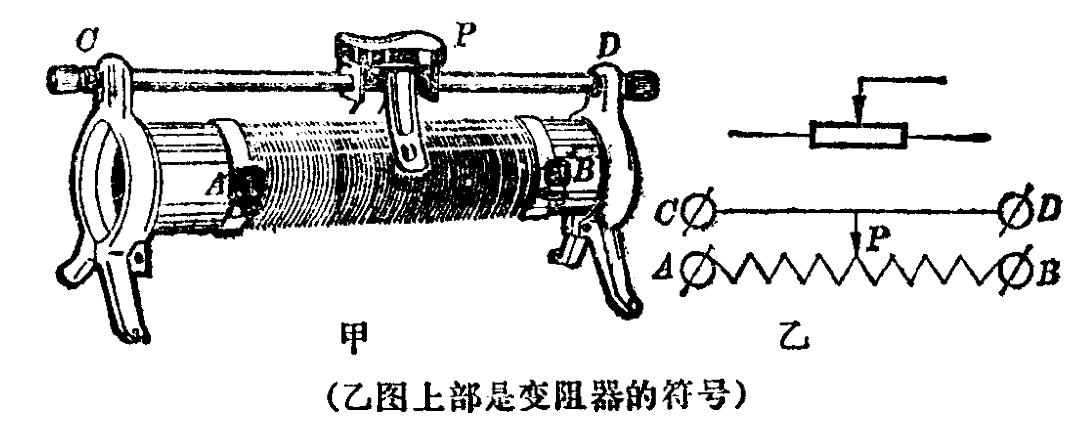
\includegraphics[width=0.7\textwidth]{../pic/czwl2-ch8-19}
    \caption{滑动变阻器(甲)和它的结构示意图(乙)}\label{fig:8-19}
\end{figure}

实验室里常用的是滑动变阻器,构造如图 \ref{fig:8-19} 所示。
在瓷筒上紧密地缠着一个线圈,线圈由表面涂着绝缘漆的合金线绕成,它的两头分别接在接线柱 $A$、$B$ 上。
瓷筒上方装着一根金属棒,棒的两端各有一个接线柱 $C$ 和 $D$,棒上还套着一个可以滑动的接触器,
它的金属滑片 $P$ 紧压在线圈上。线圈上能跟滑片接触的地方,绝缘漆已经刮去。

如果把电路的两头分别接在接线柱 $A$ 和金属棒两端的任意一个接线柱 $C$ 或 $D$ 上,滑片 $P$ 左边的合金线就连入了电路;
如果把电路的两头分别接在接线柱 $B$ 和金属棒两端的任意一个接线柱 $C$ 或 $D$ 上,滑片 $P$ 右边的合金线就连入了电路。
移动滑片 $P$ 的时候,连入电路的合金线的长度改变,电阻也就跟着改变。
照图 \ref{fig:8-20} 所示那样,把电池组、小灯泡、滑动变阻器、电键、安培表等连接好,移动滑片,
从安培表示数的变化,可以了解变阻器的作用。

\begin{figure}[htbp]
    \centering
    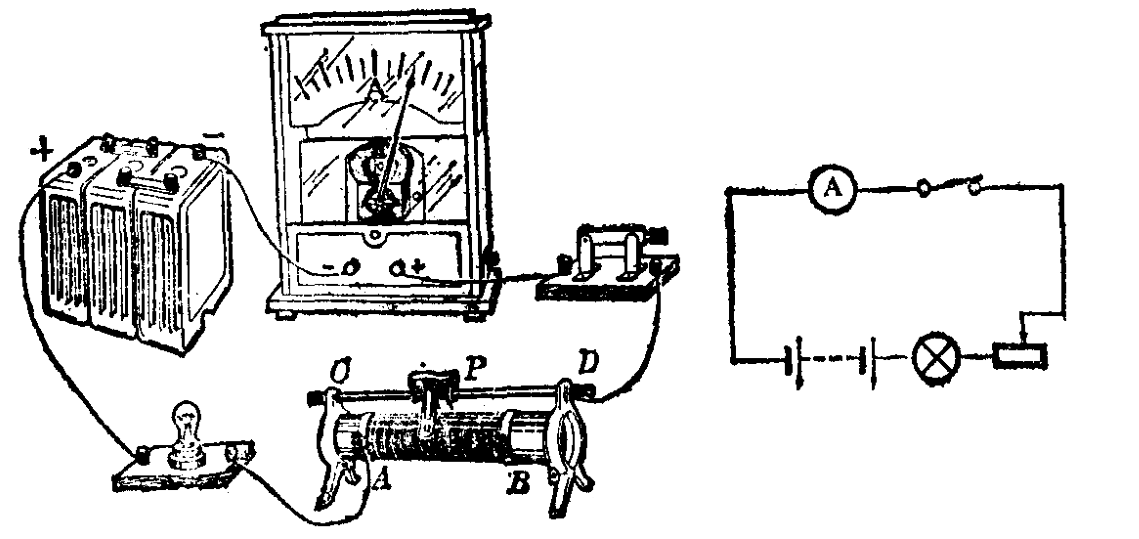
\includegraphics[width=0.7\textwidth]{../pic/czwl2-ch8-20}
    \caption{观察滑动变阻器的作用}\label{fig:8-20}
\end{figure}

变阻器在生产技术上有重要的应用。
例如,调节收音机的音量大小的电位器,实际上就是变阻器。

滑动变阻器能够逐渐地改变连入电路的电阻,但不能准确表示出连入的电阻值。
如果需要知道连入电路的电阻的准确值,就要用电阻箱。

\begin{figure}[htbp]
    \centering
    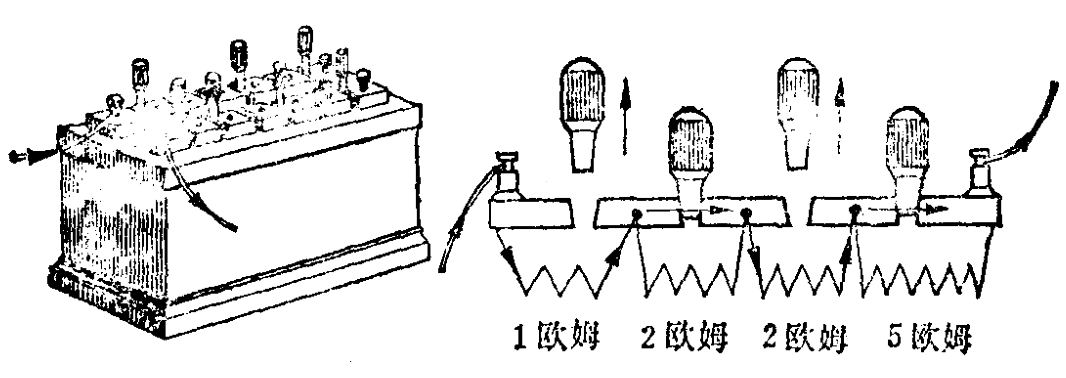
\includegraphics[width=0.7\textwidth]{../pic/czwl2-ch8-21}
    \caption{电阻箱(左)和它的结构示意图(右)}\label{fig:8-21}
\end{figure}


电阻箱(图 \ref{fig:8-21})的盖上有一排铜块,铜块间有插孔,孔里插铜塞。
当铜塞插在孔里时,就把相邻的两个铜块连在一起,电流就由铜块上通过。
当铜塞拨出时,电流就通过插孔下面的合金线。
拨出的铜塞越多,连入电路的合金线就越长,电阻也越大。
每个插孔下的合金线的电阻值都标在插孔旁。
只要把未插铜塞的插孔旁的数值加在一起,就是连入电路的电阻值。
图 \ref{fig:8-21} 右图表示连入电路的电阻值是 $1\oumu + 2\oumu = 3\oumu$。


